\documentclass{standalone}
\usepackage{tikz}
\usetikzlibrary{patterns, positioning}
\usepackage[sfdefault]{ClearSans} %% option 'sfdefault' activates Clear Sans as the default text font
\usepackage[T1]{fontenc}

\begin{document}
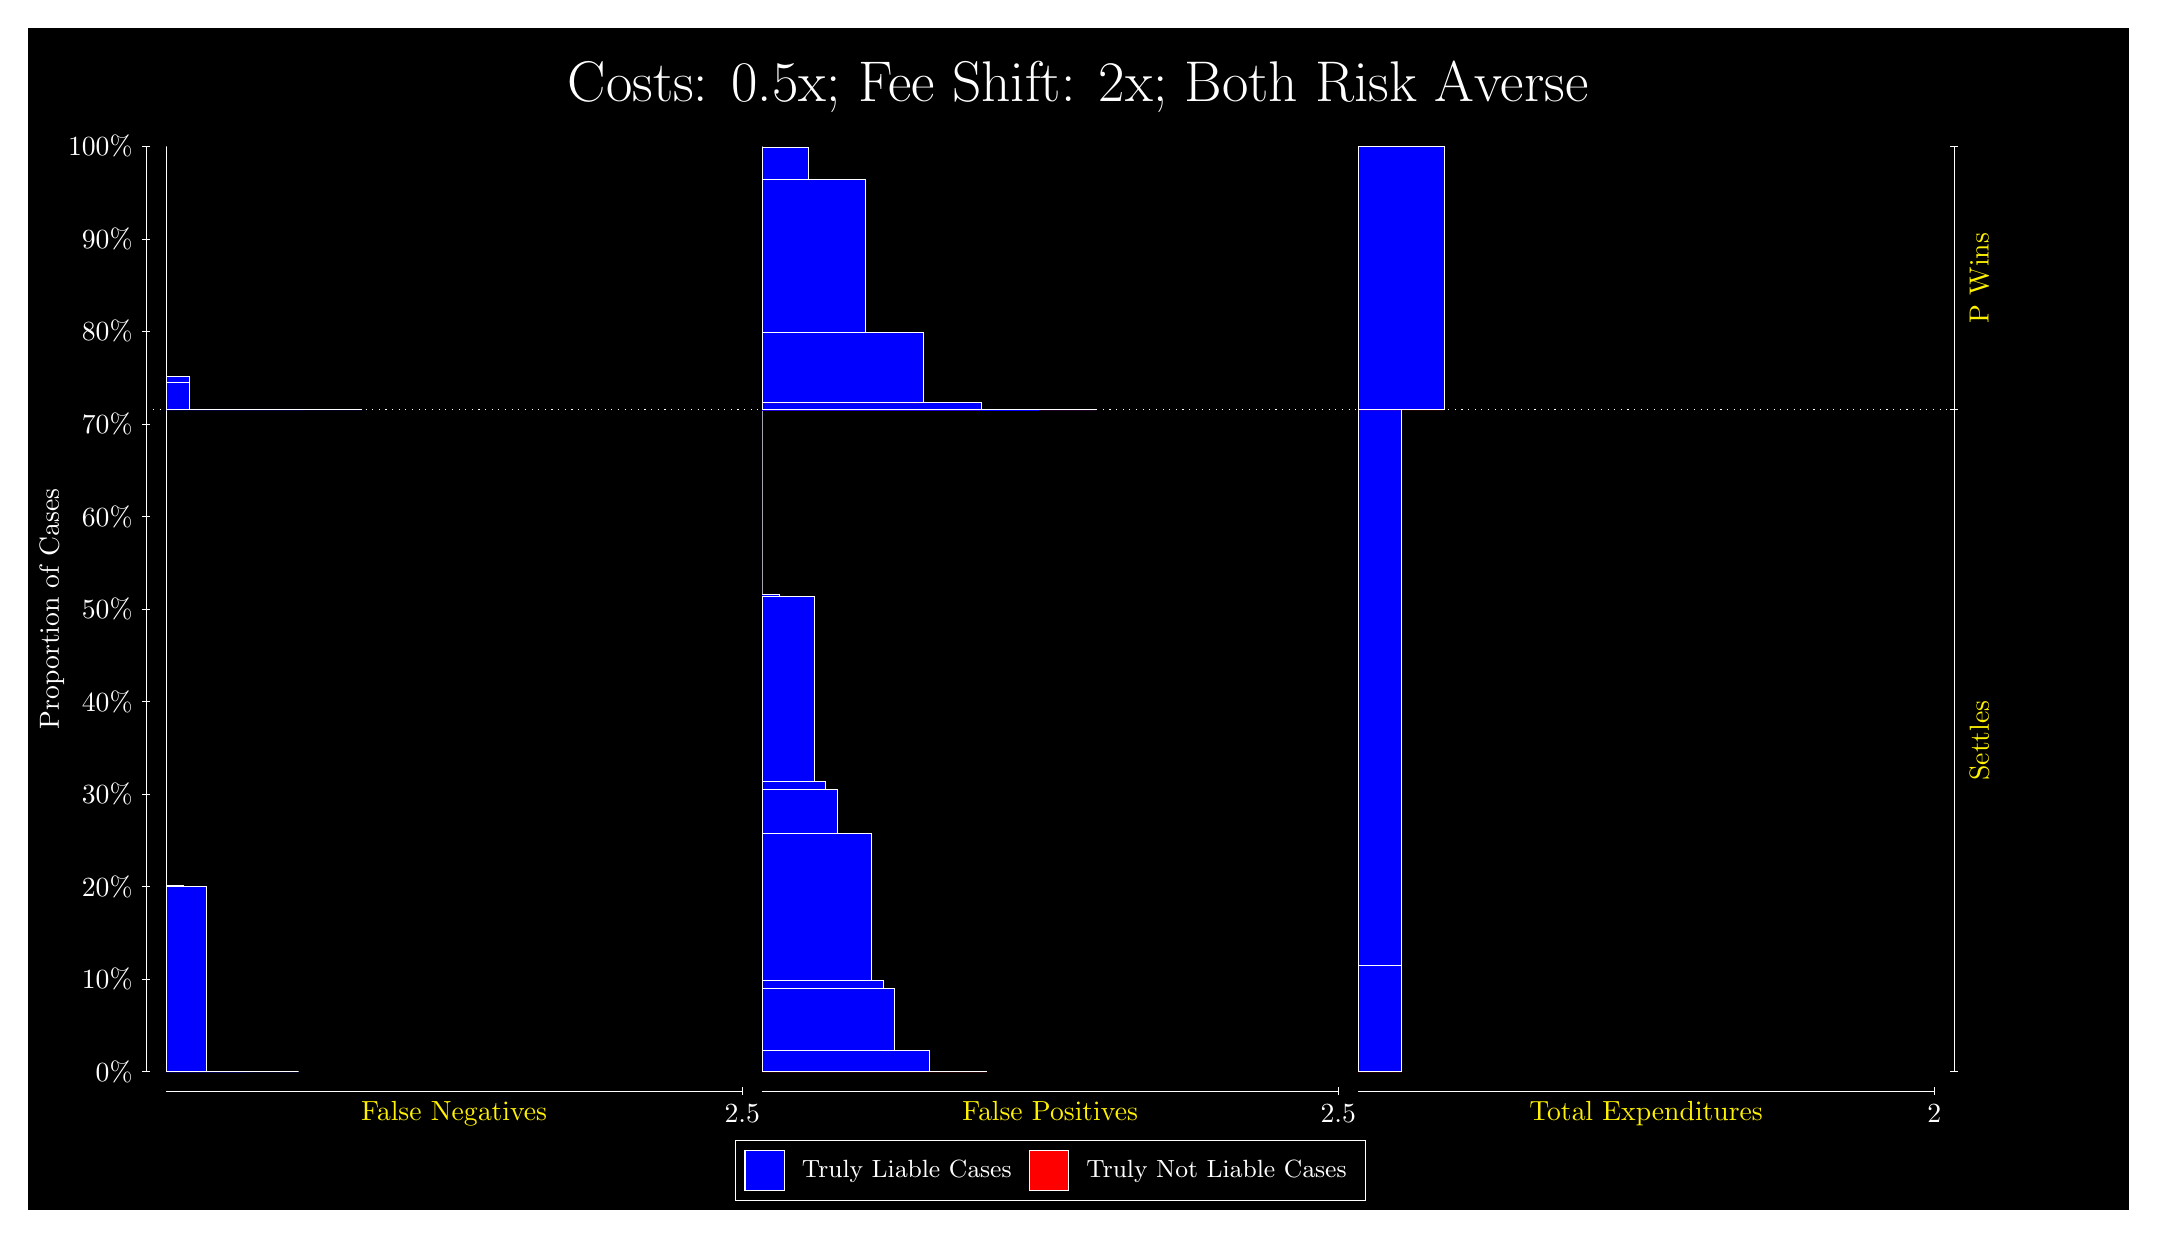
\begin{tikzpicture}
\draw[fill=black] (0,0) rectangle (26.667,15);
\draw[text=white] (0,13.5) rectangle (26.667,15) node[midway] {\huge Costs: 0.5x; Fee Shift: 2x; Both Risk Averse};
\draw[white, very thin] (1.5,1.75) -- (1.5,13.5);
\node[rotate=90, text=white, anchor=center] at (0.3, 7.625) {Proportion of Cases};
\draw[white, very thin] (1.45,1.75) -- (1.55,1.75);
\node[text=white, anchor=east] at (1.45, 1.75) {0\%};
\draw[white, very thin] (1.45,2.925) -- (1.55,2.925);
\node[text=white, anchor=east] at (1.45, 2.925) {10\%};
\draw[white, very thin] (1.45,4.1) -- (1.55,4.1);
\node[text=white, anchor=east] at (1.45, 4.1) {20\%};
\draw[white, very thin] (1.45,5.275) -- (1.55,5.275);
\node[text=white, anchor=east] at (1.45, 5.275) {30\%};
\draw[white, very thin] (1.45,6.45) -- (1.55,6.45);
\node[text=white, anchor=east] at (1.45, 6.45) {40\%};
\draw[white, very thin] (1.45,7.625) -- (1.55,7.625);
\node[text=white, anchor=east] at (1.45, 7.625) {50\%};
\draw[white, very thin] (1.45,8.8) -- (1.55,8.8);
\node[text=white, anchor=east] at (1.45, 8.8) {60\%};
\draw[white, very thin] (1.45,9.975) -- (1.55,9.975);
\node[text=white, anchor=east] at (1.45, 9.975) {70\%};
\draw[white, very thin] (1.45,11.15) -- (1.55,11.15);
\node[text=white, anchor=east] at (1.45, 11.15) {80\%};
\draw[white, very thin] (1.45,12.325) -- (1.55,12.325);
\node[text=white, anchor=east] at (1.45, 12.325) {90\%};
\draw[white, very thin] (1.45,13.5) -- (1.55,13.5);
\node[text=white, anchor=east] at (1.45, 13.5) {100\%};

\draw[white, very thin] (24.457,1.75) -- (24.457,13.5);
\draw[white, very thin] (24.407,1.75) -- (24.507,1.75);
\node[anchor=west] at (24.407, 1.75) {};
\draw[white, very thin] (24.407,10.156) -- (24.507,10.156);
\node[anchor=west] at (24.407, 10.156) {};
\draw[white, very thin] (24.407,13.5) -- (24.507,13.5);
\node[anchor=west] at (24.407, 13.5) {};

\draw[white, very thin, fill=blue] (1.75,1.75) rectangle (3.4333,1.75);
\draw[white, very thin, fill=blue] (1.75,1.75) rectangle (2.8478,1.75);
\draw[white, very thin, fill=blue] (1.75,1.75) rectangle (2.7015,1.75);
\draw[white, very thin, fill=blue] (1.75,1.75) rectangle (2.2623,4.0999);
\draw[white, very thin, fill=blue] (1.75,4.0999) rectangle (2.1159,4.101);
\draw[white, very thin, fill=blue] (1.75,4.101) rectangle (1.9696,4.1207);
\draw[white, very thin, fill=red] (1.75,4.1207) rectangle (1.75,4.1207);
\draw[white, very thin, fill=blue] (1.75,4.1207) rectangle (1.75,10.156);
\draw[white, very thin, fill=blue] (1.75,10.156) rectangle (4.2384,10.156);
\draw[white, very thin, fill=blue] (1.75,10.156) rectangle (3.5065,10.156);
\draw[white, very thin, fill=blue] (1.75,10.156) rectangle (2.7746,10.164);
\draw[white, very thin, fill=blue] (1.75,10.164) rectangle (2.0428,10.498);
\draw[white, very thin, fill=blue] (1.75,10.498) rectangle (2.0428,10.58);
\draw[white, very thin, fill=red] (1.75,10.58) rectangle (1.75,10.58);
\draw[white, very thin, fill=blue] (1.75,10.58) rectangle (1.75,13.5);
\draw[white, very thin, fill=red] (9.3189,1.75) rectangle (12.173,1.75);
\draw[white, very thin, fill=blue] (9.3189,1.75) rectangle (12.173,1.7525);
\draw[white, very thin, fill=red] (9.3189,1.7525) rectangle (11.588,1.7525);
\draw[white, very thin, fill=blue] (9.3189,1.7525) rectangle (11.588,1.7538);
\draw[white, very thin, fill=blue] (9.3189,1.7538) rectangle (11.441,2.0224);
\draw[white, very thin, fill=red] (9.3189,2.0224) rectangle (11.002,2.0224);
\draw[white, very thin, fill=blue] (9.3189,2.0224) rectangle (11.002,2.8033);
\draw[white, very thin, fill=blue] (9.3189,2.8033) rectangle (10.856,2.9079);
\draw[white, very thin, fill=blue] (9.3189,2.9079) rectangle (10.709,4.7806);
\draw[white, very thin, fill=blue] (9.3189,4.7806) rectangle (10.27,5.3348);
\draw[white, very thin, fill=blue] (9.3189,5.3348) rectangle (10.124,5.4393);
\draw[white, very thin, fill=blue] (9.3189,5.4393) rectangle (9.9776,7.7851);
\draw[white, very thin, fill=blue] (9.3189,7.7851) rectangle (9.5384,7.8048);
\draw[white, very thin, fill=blue] (9.3189,7.8048) rectangle (9.3921,7.8059);
\draw[white, very thin, fill=blue] (9.3189,7.8059) rectangle (9.3189,10.156);
\draw[white, very thin, fill=red] (9.3189,10.156) rectangle (13.564,10.156);
\draw[white, very thin, fill=blue] (9.3189,10.156) rectangle (13.564,10.156);
\draw[white, very thin, fill=red] (9.3189,10.156) rectangle (12.832,10.156);
\draw[white, very thin, fill=blue] (9.3189,10.156) rectangle (12.832,10.157);
\draw[white, very thin, fill=red] (9.3189,10.157) rectangle (12.1,10.157);
\draw[white, very thin, fill=blue] (9.3189,10.157) rectangle (12.1,10.244);
\draw[white, very thin, fill=red] (9.3189,10.244) rectangle (11.368,10.244);
\draw[white, very thin, fill=blue] (9.3189,10.244) rectangle (11.368,11.142);
\draw[white, very thin, fill=red] (9.3189,11.142) rectangle (10.636,11.142);
\draw[white, very thin, fill=blue] (9.3189,11.142) rectangle (10.636,13.076);
\draw[white, very thin, fill=blue] (9.3189,13.076) rectangle (9.9044,13.492);
\draw[white, very thin, fill=blue] (9.3189,13.492) rectangle (9.3189,13.5);
\draw[white, very thin, fill=red] (16.888,1.75) rectangle (17.437,1.75);
\draw[white, very thin, fill=blue] (16.888,1.75) rectangle (17.437,3.1048);
\draw[white, very thin, fill=red] (16.888,3.1048) rectangle (17.437,3.1048);
\draw[white, very thin, fill=blue] (16.888,3.1048) rectangle (17.437,10.156);
\draw[white, very thin, fill=red] (16.888,10.156) rectangle (17.986,10.156);
\draw[white, very thin, fill=blue] (16.888,10.156) rectangle (17.986,10.165);
\draw[white, very thin, fill=red] (16.888,10.165) rectangle (17.986,10.165);
\draw[white, very thin, fill=blue] (16.888,10.165) rectangle (17.986,13.5);
\draw[white, dotted] (1.5,10.156) -- (24.457,10.156);
\draw[white, very thin] (1.75,1.5) -- (9.0689,1.5);
\node[text=yellow, anchor=north] at (5.4094, 1.5) {False Negatives};
\draw[white, very thin] (9.0689,1.45) -- (9.0689,1.55);
\node[text=white, anchor=north] at (9.0689, 1.45) {2.5};

\draw[white, very thin] (9.3189,1.5) -- (16.638,1.5);
\node[text=yellow, anchor=north] at (12.978, 1.5) {False Positives};
\draw[white, very thin] (16.638,1.45) -- (16.638,1.55);
\node[text=white, anchor=north] at (16.638, 1.45) {2.5};

\draw[white, very thin] (16.888,1.5) -- (24.207,1.5);
\node[text=yellow, anchor=north] at (20.547, 1.5) {Total Expenditures};
\draw[white, very thin] (24.207,1.45) -- (24.207,1.55);
\node[text=white, anchor=north] at (24.207, 1.45) {2};

\node[text=yellow, centered, rotate=90] at (24.777, 5.9529) {Settles};
\node[text=yellow, centered, rotate=90] at (24.777, 11.828) {P Wins};

\draw (12.978300999999998,1.5) node[draw=none] (baseCoordinate) {};
\begin{scope}[align=center]
        \matrix[scale=0.5, draw=white, below=0.5cm of baseCoordinate, nodes={draw}, column sep=0.1cm]{
            \node[rectangle, draw, minimum width=0.5cm, minimum height=0.5cm, fill=blue] {}; &
            \node[draw=none, font=\small, text=white] (B) {Truly Liable Cases}; &
            \node[rectangle, draw, minimum width=0.5cm, minimum height=0.5cm, fill=red] {}; &
            \node[draw=none, font=\small, text=white] (B) {Truly Not Liable Cases}; \\
            };
\end{scope}

\end{tikzpicture}
\end{document}